\documentclass{article}
\usepackage{amsmath}
\usepackage{tikz}
\usepackage{mathtools}
\usepackage{enumitem}
\usepackage[a4paper, total={6in, 8in}]{geometry}
\usepackage{amssymb}
\usepackage{color}
\usepackage{lscape}
\usepackage{ifthen}
\usepackage{listings}
\usepackage{xcolor}
\usepackage{float}
\usepackage{hyperref}
\usepackage{fancyhdr}
\pagestyle{fancy}

\numberwithin{equation}{section}

% Define the header
\fancyfoot[L]{ECMA 31380 - Causal Machine Learning}
\fancyfoot[R]{Fernando Urbano}
\renewcommand{\footrulewidth}{0.2pt}
\fancyhead[L]{}
\fancyhead[C]{Comparative Analysis of DML Methods Across Causal Inference Frameworks}
\fancyhead[R]{}

\usepackage{graphicx}
\setlength{\parskip}{0.5em}
\setlength{\parindent}{0pt}
\renewcommand{\thesubsection}{\thesection.\arabic{subsection}}
\newcommand{\divider}{\vspace{1em}\hrule\vspace{1em}}

\definecolor{codegreen}{rgb}{0, 0.6, 0}
\definecolor{codegray}{rgb}{0.5, 0.5, 0.5}
\definecolor{codepurple}{rgb}{0.58, 0, 0.82}
\definecolor{backcolour}{rgb}{0.95, 0.95, 0.92}
\newenvironment{colorparagraph}[1]{\par\color{#1}}{\par}
\definecolor{questioncolor}{RGB}{20, 40, 150}
\definecolor{annotationcolor}{RGB}{20, 200, 20}
\definecolor{tacolor}{RGB}{200, 0, 0}

\title{Comparative Analysis of Double Machine Learning Methods Across Causal Inference Frameworks}
\author{Fernando Rocha Urbano}
\date{Autumn 2024}

\newboolean{bool:showfrontdooradjustment}
\newboolean{bool:showquestions}
\newboolean{bool:showannotations}

\setboolean{bool:showfrontdooradjustment}{false}
\setboolean{bool:showquestions}{true}
\setboolean{bool:showannotations}{true}

\lstdefinestyle{Python}{
    backgroundcolor=\color{backcolour},   
    commentstyle=\color{codegreen},
    keywordstyle=\color{magenta},
    numberstyle=\tiny\color{codegray},
    stringstyle=\color{codepurple},
    basicstyle=\ttfamily\footnotesize,
    breakatwhitespace=false,         
    breaklines=true,                 
    captionpos=b,                    
    keepspaces=true,                 
    numbers=left,                    
    numbersep=5pt,                  
    showspaces=false,                
    showstringspaces=false,
    showtabs=false,                  
    tabsize=2
}

\usetikzlibrary{arrows.meta, positioning}

\begin{document}

\maketitle

\section{Goal}

The goal of this project is to evaluate the performance of different Double Machine Learning (DML) models in recovering the Average Treatment Effect (ATE) across various causal inference scenarios addressed in simulations.

Ideally, the project should provide actionable recommendations for selecting the most appropriate DML method based on the causal scenario, data generating process (linear vs. non-linear), noise levels, sample size, sparsity of causal covariates, number of causal and non-causal covariates. Additionally, we aim to create a benchmarking framework that practitioners can use to evaluate and compare causal inference estimates derived from the tested methods in different scenarios.

The main DML models used to evaluate are OLS, Random Forest, Neural Network, LASSO, and Elastic Net with correct and incorrect specifications. The causal scenario evaluated (which are based on different data generating processes) are Backdoor Path, Frontdoor Path, and Instrumental Variables. Covariates dimension, noise levels, and sample size are also varied to evaluate differences in performance for each combination of scenario, model, and specification.

The main metric evaluated is the capacity to recover the true Average Treatment Effect (ATE) in each scenario. In order to achieve this goal, we calculate bias, variance, mean squared error (MSE) and confidence interval coverage of the ATE estimates.

Below, we highlight some of the questions we are able to answer with the proposed simulations:
\begin{enumerate}[label=\arabic*.]
    \item Which model performs better for different ratio of number of causal ($d_c$) and non-causal covariates ($d_a$)?
    \item Which model performs better for high-dimensional data?
    \item Which model performs better for each of the causal inference scenarios (Backdoor, Frontdoor, and IV)?
    \item Which model performs better overall for the estimation of treatment, outcome, and instrument?
    \item Which model has the best convergence rate?
    \item Which model performs better for different noise levels ($\sigma_z$, $\sigma_t$, $\sigma_y$)?
    \item Do bias, variance, MSE and confidence interval coverage metrics point to the same ranking of models?
    \item Which model performs better for different levels of sparsity between covariates (level of correlation between covariates)?
    \item Which model performs better when there is misspecification in the nuisance functions?
    \item Which model performs better when there is unobserved confounders ($U_i$) not corrected by instrument (a type of misspecification)?
\end{enumerate}

\section{Double Machine Learning}

\ifthenelse{\boolean{bool:showannotations}}{
\begin{colorparagraph}{annotationcolor}
    Brief introduction of DML history
\end{colorparagraph}
}

\subsection{Problem Setup}

Consider a random sample ${(Y_i, T_i, X_i)}_{i=1}^n$, where $Y_i \in \mathbb{R}$ is the outcome variable, $T_i \in {0,1}$ is a binary treatment indicator, and $X_i \in \mathbb{R}^d$ is a vector of covariates.

Our goal is to estimate the Average Treatment Effect (ATE), defined as:
\begin{equation}
\tau = \mathbb{E}[Y_i(1) - Y_i(0)],
\label{eq:tau_hat_potential_outcome}
\end{equation}
where $Y_i(t)$ denotes the potential outcome for unit $i$ under treatment $T_i = t$.

\ifthenelse{\boolean{bool:showannotations}}{
\begin{colorparagraph}{annotationcolor}
    Probably expand explanation on this section, specifically on the issues in achieving potential outcome estimates.
\end{colorparagraph}
}

\subsection{Identification via Conditional Expectations}

Under the Conditional Independence Assumption (CIA) and overlap conditions, the ATE can be identified as:
\begin{equation}
\tau = \mathbb{E}[\mu_1(X_i) - \mu_0(X_i)],
\label{eq:tau_hat_potential_outcome_diff_means}
\end{equation}
where $\mu_t(X_i) = \mathbb{E}[Y_i | T_i = t, X_i]$ is the conditional expectation of the outcome given treatment and covariates.

\subsection{DML Estimator}

The DML framework aims to estimate $\tau$ while controlling for high-dimensional or complex relationships between $Y_i$, $T_i$, and $X_i$. The key idea is to use machine learning methods to estimate the nuisance parameters and then construct an estimator for $\tau$ that is robust to estimation errors in these nuisance parameters.

\ifthenelse{\boolean{bool:showannotations}}{
\begin{colorparagraph}{annotationcolor}
    More explanation on what are nuisance functions.
\end{colorparagraph}
}

\subsubsection{Nuisance Parameter Estimation}

We define the following nuisance functions:
\begin{align}
& m(X_i) = \mathbb{E}[Y_i | X_i],
\label{eq:m_x_for_target}
\\
& g(X_i) = \mathbb{E}[T_i | X_i],
\label{eq:g_x_for_treatment}
\\
& \pi(X_i) = \mathbb{P}(T_i = 1 | X_i) \quad \text{(propensity score)}
\label{eq:pi_x_for_treatment}
\end{align}

These functions can be estimated using flexible machine learning methods such as LASSO, Random Forests, or Neural Networks.

Under mild regularity conditions and appropriate rates of convergence for the nuisance estimators, the DML estimator is root-n consistent and asymptotically normal (we make the regularity conditions explicity in Appendix~\ref{subsec:appendix_mild_regularity_conditions_for_dml}). DML provides valid confidence intervals and hypothesis tests even when using complex machine learning methods for $\hat{m}(X)$ and $\hat{g}(X)$.

\subsubsection{Orthogonal Score Function}

To achieve robustness, we construct an orthogonal score function $\psi(Y_i, T_i, X_i; \eta)$, where $\eta = (m, g)$ represents the nuisance parameters. The orthogonal score satisfies the Neyman orthogonality condition, which ensures that small estimation errors in $\eta$ have a negligible first-order impact on the estimation of $\tau$.

A common choice for the orthogonal score is:
\begin{equation}
\psi(Y_i, T_i, X_i; \eta) = \left( \frac{T_i - g(X_i)}{\pi(X_i)(1 - \pi(X_i))} \right) (Y_i - m(X_i)) + \left( m_1(X_i) - m_0(X_i) \right) - \tau,
\label{eq:orthogonal_score}
\end{equation}

where $g(X_i) = \pi(X_i)$ in case of binary treatment and $m_t(X_i) = \mathbb{E}[Y_i | T_i = t, X_i]$ for $t \in \{0,1\}$.

\subsubsection{Estimation Procedure}

The estimation of DML models contains several steps:
\begin{enumerate}[label=\roman*.]
\item Estimate Nuisance Functions: Use one of the outlined ML models to obtain estimators $\hat{m}(X_i)$ and $\hat{g}(X_i)$ for the nuisance functions.

\item Compute the Score Function: Evaluate the orthogonal score $\psi(Y_i, T_i, X_i; \hat{\eta})$ using the estimated nuisance parameters.

\item Estimate $\tau$: Solve the empirical moment condition which yields $\hat{\tau}$:

\begin{equation}
\frac{1}{n} \sum_{i=1}^n \psi(Y_i, T_i, X_i; \hat{\eta}) = 0.
\label{eq:orthogonal_score_psi}
\end{equation}
\end{enumerate}

The orthogonal score function mitigates the impact of errors in $\hat{m}(X)$ and $\hat{g}(X)$ on the estimation of $\tau$ while also accomodating the use of modern ML techniques, allowing complex relationships between $Y$, $X$ and $T$.

To prevent overfitting and ensure that the estimation error in the nuisance parameters does not bias the estimator of $\tau$ we employ cross-fitting.

\subsubsection{Cross-Fitting}

The steps of cross-fitting are:

\begin{enumerate}
\item Split the Sample: Divide the data into K folds $\{\mathcal{I}_k\}{k=1}^K$.
\item For Each Fold:
\begin{enumerate}
\item Train Nuisance Estimators: Use data from all other folds:
$$
\mathcal{I}_{-k} = \bigcup{j \neq k} \mathcal{I}_j
$$
to estimate $\hat{m}^{(-k)}(X_i)$ and $\hat{g}^{(-k)}(X_i)$.

\item Compute Score Function: For observations in fold $\mathcal{I}_k$, compute $\psi(Y_i, T_i, X_i; \hat{\eta}^{(-k)})$ using the nuisance estimates from step (a):

\begin{equation}
    \begin{split}
        \psi(Y_i, T_i, X_i; \hat{\eta}^{(-k)}) = & \left( \frac{T_i - \hat{g}^{(-k)}(X_i)}{\hat{\pi}^{(-k)}(X_i)} \right) (Y_i - \hat{m}^{(-k)}(X_i)) \\
        & + \ \hat{m}_1^{(-k)}(X_i) - \hat{m}_0^{(-k)}(X_i) - \tau^{(-k)}.
    \end{split}
    \label{eq:orthogonal_score_fold_k}
\end{equation}

\end{enumerate}
\item Aggregate: Combine the estimates from all folds:

\begin{equation}
\hat{\tau} = \frac{1}{n} \sum_{k=1}^K \sum_{i \in \mathcal{I}_k} \hat{\tau}_i^{(-k)} =  \frac{1}{K} \sum_{k=1}^K \hat{\tau}^{(-k)}
\label{eq:avg_tau_hat}
\end{equation}

\end{enumerate}

\section{Causal Inference Scenarios}

The three most relevant scenarios of causal inference are the ones that require Instrumental Variables, Backdoor Adjustment, or Front Door Adjustment. A common way to represent the causal relation related to those is through the use of DAGs.

\subsection{DAG (Directed Acyclic Graph)}

Directed Acyclic Graph (DAG) serves as a representation of causal assumptions and a tool for deriving statistical properties of the variables involved.

It is composed of nodes (vertices) representing random variables or features and directed edges (arrows), indicating a direct influence or causal effect of $T$ on $Y$.

\begin{figure}[H]
    \centering
    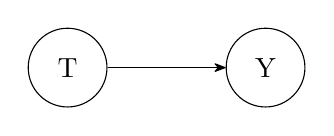
\begin{tikzpicture}[
        >={Stealth[round]},
        every node/.style={draw, circle, minimum size=1cm},
        every edge/.style={draw, ->, thick},
        node distance=2cm
    ]
    
    \node (T) {T};
    \node (Y) [right=of T, xshift=-0.5cm] {Y};
    
    \draw[->] (T) -- (Y);
    \end{tikzpicture}
    \caption{DAG Example}
    \label{fig:dag_example}
\end{figure}

The acyclic characterist is due to absence of directed cycles; that is, there is no path where you can start at a node $X$ and, by following directed edges, return to $X$.

\subsection{Backdoor Adjustment}

A backdoor path from treatment $T$ to the outcome $Y$ represents alternative routes through which association can flow from $T$ to $Y$ that are not due to the causal effect of $T$ on $Y$. In the representation, the confounder $C$ is a common cause of both $T$ and $Y$, thus, a backdoor path.

In such case, the association between $T$ and $Y$ may be partially or entirely due to their mutual dependence on $C$ rather than a direct causal effect, leading to biased causal estimates of the treatment if $C$ is ignored.

The causal effect of $T$ on $Y$ can be expressed using the backdoor adjustment formula:

\begin{equation}
    \mathbb{P}[Y(t)] = \sum_C \mathbb{P}[Y \mid T, C] \mathbb{P}[C],
\end{equation}

Which serves a markov factorization, calculating with respect to the DAG structure.

For the backdoor adjustment to be valid, the following conditions must be satisfied:

\begin{enumerate}
    \item No variable in the adjustment set is a descendant of the treatment $T$.
    \item The adjustment set blocks all backdoor paths from $T$ to $Y$ (backdoor path is any path from $T$ to $Y$ that starts with an arrow into $T$).
\end{enumerate}

DAG~\ref{fig:dag_backdoor_path} illustrates the backdoor path involving the confounder $C$, treatment $T$, outcome $Y$, and features with non-causal association $X_a$ which would not be present in a typical backdoor adjustment DAG, but play a relevant role in the simulations proposed.

\begin{figure}[H]
    \centering
    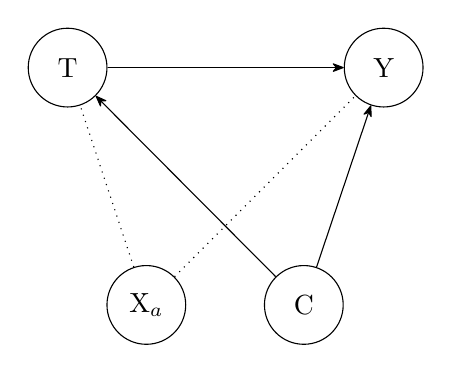
\begin{tikzpicture}[
        >={Stealth[round]},
        every node/.style={draw, circle, minimum size=1cm},
        every edge/.style={draw, ->, thick},
        node distance=2cm
    ]
    
    \node (T) {T};
    % \node (C) [above=of T, xshift=1.5cm] {C};
    \node (Y) [right=of T, xshift=1cm] {Y};
    \node (XC) [below=of T, xshift=3cm] {$\text{C}$};
    \node (XA) [below=of T, xshift=1cm] {$\text{X}_a$};
    
    % \draw[->] (C) -- (T);
    % \draw[->] (C) -- (Y);
    \draw[->] (T) -- (Y);  
    \draw[->] (XC) -- (T);
    \draw[->] (XC) -- (Y);
    \draw[dotted] (XA) -- (T);
    \draw[dotted] (XA) -- (Y);
    \end{tikzpicture}
    \caption{DAG of Backdoor Path}
    \label{fig:dag_backdoor_path}
\end{figure}

\subsubsection{Backdoor Adjustment Scenario in DML}

In Backdoor Adjustment with DML, the ideal $m(X_i) = \mathbb{E}[Y_i | X_i]$ and $g(X_i) = \mathbb{E}[T_i | X_i]$ from Equations \eqref{eq:m_x_for_target} and \eqref{eq:g_x_for_treatment} are:

\begin{align}
    & m_{\text{BA}}(C_i) = \mathbb{E}[Y_i | C_i],
    \label{eq:m_x_for_target_backdoor_adjustment}
    \\
    & g_{\text{BA}}(C_i) = \mathbb{E}[T_i | C_i],
    \label{eq:g_x_for_treatment_backdoor_adjustment}
\end{align}

In our simulations we also test the habilit of the ML models to estimate ATE under the following scenarios. In these scenarios, the superscript $\text{w}_i$ on the nuisance functions denotes the i-th scenario which involves misspecifications of the nuisance functions.

\paragraph{Inclusion of $C_i$ and $X_{a, i}$ on every nuisance function}

\begin{align}
    & m_{\text{BA}}^{\text{w}_1}(C_i, X_{a, i}) = \mathbb{E}[Y_i | C_i, X_{a, i}],
    \label{eq:m_x_for_target_backdoor_adjustment_wrong_1}
    \\
    & g_{\text{BA}}^{\text{w}_1}(C_i, X_{a, i}) = \mathbb{E}[T_i | C_i, X_{a, i}],
    \label{eq:g_x_for_treatment_backdoor_adjustment_wrong_1}
\end{align}

Equations \eqref{eq:m_x_for_target_backdoor_adjustment_wrong_1} and \eqref{eq:g_x_for_treatment_backdoor_adjustment_wrong_1} represent a scenario in which one would not be aware that $X_a$ does not cause $T$ and $Y$.

\paragraph{Only partial inclusion of $C_i$ and inclusion of $X_{a, i}$ on every nuisance function}
\label{par:backdoor_adjustment_wrong_2}

\begin{align}
    & m_{\text{BA}}^{\text{w}_2}(C^{p}_i, X_{a, i}) = \mathbb{E}[Y_i | C^{p}_i, X_{a, i}],
    \label{eq:m_x_for_target_backdoor_adjustment_wrong_2}
    \\
    & g_{\text{BA}}^{\text{w}_2}(C^{p}_i, X_{a, i}) = \mathbb{E}[T_i | C^{p}_i, X_{a, i}],
    \label{eq:g_x_for_treatment_backdoor_adjustment_wrong_2}
\end{align}

Equations \eqref{eq:m_x_for_target_backdoor_adjustment_wrong_2} and \eqref{eq:g_x_for_treatment_backdoor_adjustment_wrong_2} also represent a scenario in which one would not be aware that $X_a$ does not cause $T$ and $Y$ and also does not include all causal cofounders. $C^{p}_i$ is subset of $C_i$ included, where $C_i \in \mathbb{R}^{d_c}$ and $C^{p}_i \in \mathbb{R}^{d_{cp}}$ and $d_c > d_{cp}$.

\ifthenelse{\boolean{bool:showfrontdooradjustment}}{
\begin{colorparagraph}{annotationcolor}
\subsection{Frontdoor Adjustment}

Frontdoor adjustment is a method used to estimate the causal effect of treatment $T$ on outcome $Y$ when there is unmeasured confounding that cannot be addressed using backdoor adjustment. It leverages a mediator $M$ that lies on the causal path from $T$ to $Y$.

The causal effect of $T$ on $Y$ can be expressed using the frontdoor adjustment formula:

\begin{equation}
\mathbb{P}[Y(t)] = \sum_M \mathbb{P}[M \mid T=t] \sum_{t’} \mathbb{P}[Y \mid M, T=t’] \mathbb{P}[T=t’].
\end{equation}

For instance, the average treatment effect in case $M, T \in \{0, 1\}$:

\begin{equation}
\tau = \left[ \mathbb{P}(M = 1 \mid T = 1) - \mathbb{P}(M = 1 \mid T = 0) \right] \times \left[ \mathbb{E}[Y \mid M = 1] - \mathbb{E}[Y \mid M = 0] \right]
\end{equation}

For the frontdoor adjustment to be valid, the following conditions must be satisfied:

\begin{enumerate}
\item All causal paths from $T$ to $Y$ pass through $M$ (i.e., there is no direct effect of $T$ on $Y$ bypassing $M$).
\item There are no unmeasured confounders between $T$ and $M$.
\item All backdoor paths from $M$ to $Y$ are blocked by $T$ (i.e., there are no unmeasured confounders between $M$ and $Y$ that are not affected by $T$).
\end{enumerate}

DAG~\ref{fig:dag_frontdoor_path} illustrates the frontdoor adjustment involving the treatment $T$, mediator $M$, outcome $Y$, observed confounders $C$ and features with no causal association $X_a$. $C$ and $X_a$ would not be present in a typical frontdoor adjustment DAG, but are included due to their relevance in the proposed simulations.

\begin{figure}[H]
    \centering
    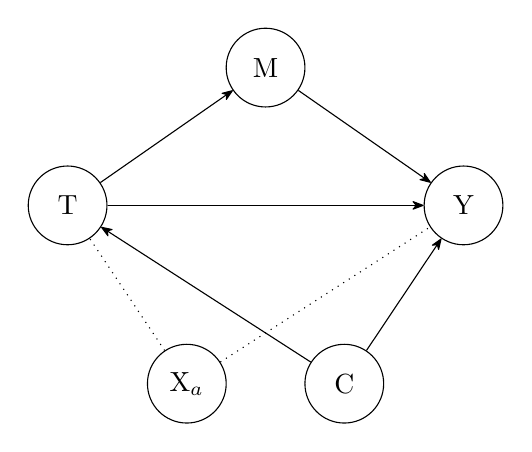
\begin{tikzpicture}[
        >={Stealth[round]},
        every node/.style={draw, circle, minimum size=1cm},
        every edge/.style={draw, ->, thick},
        node distance=2cm
    ]
    
    \node (T) {T};
    \node (M) [right=of T, xshift=-0.5cm, yshift=1.75cm] {M};
    \node (Y) [right=of M, xshift=-0.5cm, yshift=-1.75cm] {Y};
    \node (XA) [below=of M, xshift=-1cm, yshift=-1cm] {$\text{X}_a$};
    \node (XC) [below=of M, xshift=1cm, yshift=-1cm] {C};
    
    \draw[->] (T) -- (M);
    \draw[->] (M) -- (Y);
    \draw[->] (T) -- (Y);
    \draw[->] (XC) -- (T);
    \draw[->] (XC) -- (Y);
    \draw[dotted] (XA) -- (T);
    \draw[dotted] (XA) -- (Y);
    \end{tikzpicture}
    \caption{DAG of Frontdoor Path}
    \label{fig:dag_frontdoor_path}
\end{figure}

\subsubsection{Frontdoor Adjustment Scenario in DML}

In our simulations, we use a binary mediator $M_i \in \{0, 1\}$, similar to the binary treatment $T_i$.

In the Frontdoor Adjustment scenario with DML, we need to account for the mediator $M_i$ when estimating the ATE. The identification of the causal effect involves modeling the relationships between $T_i$, $M_i$, and $Y_i$.

The ideal nuisance functions for DML in this scenario are:

\begin{align}
    & m_{\text{FA}}(M_i, C_i) = \mathbb{E}[Y_i \mid M_i, C_i],
    \label{eq:m_x_for_target_frontdoor_adjustment} \\
    & h_{\text{FA}}(T_i) = \mathbb{E}(M_i \mid T_i),
    \label{eq:h_x_for_mediator_frontdoor_adjustment} \\
    & g_{\text{FA}}(C_i) = \mathbb{E}(T_i \mid C_i),
    \label{eq:g_x_for_treatment_frontdoor_adjustment}
\end{align}

Here $h_{\text{FA}}(M_i, T_i, C_i)$ is the mediator model, representing the probability of the mediator given treatment.

To adapt the orthogonal score function in the presence of the mediator, we modify Equation~\eqref{eq:orthogonal_score} to incorporate the mediator's effect. The adapted orthogonal score function is:

\begin{equation}
\psi(Y_i, T_i, M_i, C_i; \eta) = \left( \frac{T_i - g_{\text{FA}}(C_i)}{g_{\text{FA}}(C_i)(1 - g_{\text{FA}}(C_i))} \right) \left( M_i - h_{\text{FA}}(T_i) \right) \left( Y_i - m_{\text{FA}}(M_i, C_i) \right) + \delta_M \delta_Y(C_i) - \tau
\label{eq:orthogonal_score_frontdoor_adjusted}
\end{equation}

where:

\begin{align}
    \delta_M & = h_{\text{FA}}(T_i = 1) - h_{\text{FA}}(T_i = 0),
    \label{eq:delta_M_Ci} \\
    \delta_Y(C_i) & = m_{\text{FA}}(M_i = 1, C_i) - m_{\text{FA}}(M_i = 0, C_i),
    \label{eq:delta_Y_Ci}
\end{align}

and $\eta$ represents the collection of nuisance functions.

In this score function:

\begin{itemize}
    \item The first term adjusts for the treatment assignment, similar to the original score function, but now includes the mediator.
    \item The product $\left( M_i - h_{\text{FA}}(T_i) \right) \left( Y_i - m_{\text{FA}}(M_i, C_i) \right)$ captures the interaction between the mediator and the outcome.
    \item The term $\delta_M \delta_Y(C_i)$ represents the estimated causal effect based on the mediator and outcome models.
\end{itemize}

\begin{figure}[H]
    \centering
    \fbox{
        \begin{minipage}{0.99\textwidth}
            
        There are doubts about the orthogonal score function for the frontdoor adjustment.

        We are not sure if the score function should be the one presented in Equation~\eqref{eq:orthogonal_score_frontdoor_adjusted} or if it should be presented as the following:
        
        \vspace{0.3cm}
        \begin{align}
            & m_{\text{FA}}(M_i, C_i) = \mathbb{E}[Y_i \mid M_i, C_i],
            \label{eq:m_x_for_target_frontdoor_adjustment} \\
            & h_{\text{FA}}(T_i) = \mathbb{E}(M_i \mid T_i),
            \label{eq:h_x_for_mediator_frontdoor_adjustment} \\
            & g_{\text{FA}}(C_i) = \mathbb{E}(T_i \mid C_i),
            \label{eq:g_x_for_treatment_frontdoor_adjustment}
        \end{align}

        \begin{equation}
            \psi(Y_i, T_i, M_i, C_i; \eta) = \left(
                \left( \frac{M_i - h_{\text{FA}}(T_i)}{h_{\text{FA}}(T_i)(1 - h_{\text{FA}}(T_i))} \right) (Y_i - m_{\text{FA}}(M_i, C_i))
            \right) - \tau 
        \end{equation}

        \begin{equation}
            \begin{split}
                \psi(Y_i, T_i, M_i, C_i; \eta) = \\ \left(
                \left(
                    \frac{M_i - h_{\text{FA}}(T_i)}{h_{\text{FA}}(T_i)(1 - h_{\text{FA}}(T_i))}
                \right) (Y_i - m_{\text{FA}}(M_i, C_i))
                \right)
                \cdot \left(
                    h_{\text{FA}}(T_i = 1) - h_{\text{FA}}(T_i = 0)
                \right)
                - \tau
            \end{split}
        \end{equation}

        Furthermore, in the frontdoor adjustment, I am not entirely sure if $T$ should have a direct influence on $Y$. If $T$ also has a direct influence on $Y$, the DAG would look like the following:

        \begin{figure}[H]
            \centering
            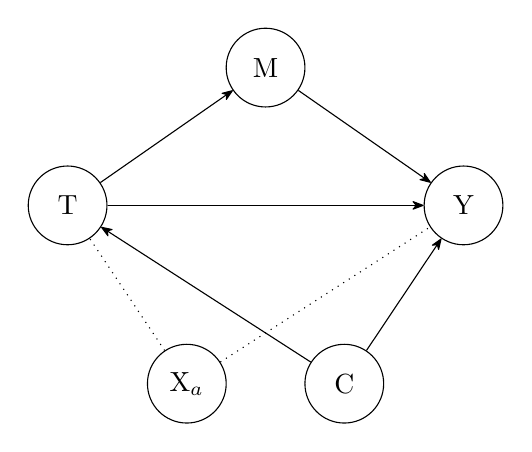
\begin{tikzpicture}[
                >={Stealth[round]},
                every node/.style={draw, circle, minimum size=1cm},
                every edge/.style={draw, ->, thick},
                node distance=2cm
            ]
            
            \node (T) {T};
            \node (M) [right=of T, xshift=-0.5cm, yshift=1.75cm] {M};
            \node (Y) [right=of M, xshift=-0.5cm, yshift=-1.75cm] {Y};
            \node (XA) [below=of M, xshift=-1cm, yshift=-1cm] {$\text{X}_a$};
            \node (XC) [below=of M, xshift=1cm, yshift=-1cm] {C};
            
            \draw[->] (T) -- (M);
            \draw[->] (M) -- (Y);
            \draw[->] (T) -- (Y);
            \draw[->] (XC) -- (T);
            \draw[->] (XC) -- (Y);
            \draw[dotted] (XA) -- (T);
            \draw[dotted] (XA) -- (Y);
            \end{tikzpicture}
            \caption{DAG of Frontdoor Path}
            \label{fig:dag_frontdoor_path}
        \end{figure}
        \vspace{0.3cm}
    \end{minipage}
    }
\end{figure}

In our simulations we also test the hability of the ML models to estimate ATE under the following scenario.

\paragraph{Inclusion of $C_i$ and $X_{a, i}$ on every nuisance function}

\begin{align}
    & m_{\text{FA}}^{\text{w}_1}(M_i, C_i, X_{a, i}) = \mathbb{E}[Y_i \mid M_i, C_i, X_{a, i}],
    \label{eq:m_x_for_target_frontdoor_adjustment_wrong_1} \\
    & h_{\text{FA}}^{\text{w}_1}(T_i, C_i, X_{a, i}) = \mathbb{E}(M_i \mid C_i, X_{a, i}),
    \label{eq:h_x_for_mediator_frontdoor_adjustment_wrong_1} \\
    & g_{\text{FA}}^{\text{w}_1}(C_i, X_{a, i}) = \mathbb{E}(T_i \mid C_i, X_{a, i}),
    \label{eq:g_x_for_treatment_frontdoor_adjustment_wrong_1}
\end{align}

Equations \eqref{eq:m_x_for_target_frontdoor_adjustment_wrong_1}, \eqref{eq:h_x_for_mediator_frontdoor_adjustment_wrong_1}, and \eqref{eq:g_x_for_treatment_frontdoor_adjustment_wrong_1} represent a scenario where one is unaware that $X_{a, i}$ has no causal relation to $T_i$, $M_i$, or $Y_i$. Equation \eqref{eq:h_x_for_mediator_frontdoor_adjustment_wrong_1} represents scenarion where one is unaware that $C$ has no causal relation to $M_i$.

\paragraph{Ignoring the mediator $M_i$}

\begin{align}
    & m_{\text{FA}}^{\text{w}_2}(C_i, X_{a, i}) = \mathbb{E}[Y_i \mid C_i, X_{a, i}],
    \label{eq:m_x_for_target_frontdoor_adjustment_wrong_2} \\
    & g_{\text{FA}}^{\text{w}_2}(C_i, X_{a, i}) = \mathbb{E}[T_i \mid C_i, X_{a, i}],
    \label{eq:g_x_for_treatment_frontdoor_adjustment_wrong_2}
\end{align}

Equations \eqref{eq:m_x_for_target_frontdoor_adjustment_wrong_2} and \eqref{eq:g_x_for_treatment_frontdoor_adjustment_wrong_2} represent a scenario where the mediator $M_i$ is unavailable or ignored and one is unaware that $X_{a, i}$ has no causal relationship to $T$ or $Y$. In this case, the orthogonal score function is the same as in Equation~\eqref{eq:orthogonal_score}.

\paragraph{Considering the mediator $M_i$ as a normal covariate}

\begin{align}
    & m_{\text{FA}}^{\text{w}_3}(C_i, M_i, X_{a, i}) = \mathbb{E}[Y_i \mid C_i, M_i, X_{a, i}],
    \label{eq:m_x_for_target_frontdoor_adjustment_wrong_3} \\
    & g_{\text{FA}}^{\text{w}_3}(C_i, M_i, X_{a, i}) = \mathbb{E}[T_i \mid C_i, M_i, X_{a, i}],
    \label{eq:g_x_for_treatment_frontdoor_adjustment_wrong_3}
\end{align}

Equations \eqref{eq:m_x_for_target_frontdoor_adjustment_wrong_3} to \eqref{eq:g_x_for_treatment_frontdoor_adjustment_wrong_3} also represent scenarios where one is unaware that $X_{a, i}$ has no causal relation to $T_i$ or $Y_i$, and the scenario where $M_i$ is available but not recognized as a mediator. In this case, the orthogonal score function is the same as in Equation~\eqref{eq:orthogonal_score}.

\end{colorparagraph}
}

\subsection{Instrumental Variable}

Instrumental variable (IV) estimation is a method used to estimate the causal effect of a treatment $T_i$ on an outcome $Y_i$ when there is unmeasured confounding $U_i$ that cannot be addressed using backdoor or frontdoor adjustments. This method leverages an instrument $Z_i$, which influences the treatment $T_i$ but has no direct effect on the outcome $Y_i$  except through $T_i$, and is independent of any unmeasured confounders $U_i$ affecting both $T_i$ and $Y_i$.

For the instrumental variable method to be valid, the following conditions must be satisfied:

\begin{enumerate}
\item Relevance: The instrument $Z$ is associated with the treatment  $T$  (i.e.,  $\text{Cov}(Z, T) \neq 0$  or \( Z \not\!\perp\!\!\!\perp T \)).
\item Exclusion Restriction: The instrument $Z$ affects the outcome $Y$ only through its effect on the treatment $T$ (i.e., there is no direct effect of $Z$ on $Y$ and no other pathways from $Z$ to $Y$ except through  $T$).
\item Independence (Ignorability): The instrument $Z$ is independent of any unmeasured confounders $U$ that affect both $T$ and $Y$ $(i.e.,  Z \perp\!\!\!\perp U )$.
\end{enumerate}

DAG~\ref{fig:dag_instrumental_variable} illustrates the instrumental variable setup involving the unobserved confounder $U$, instrument $Z$, treatment $T$, outcome $Y$, observed confounder $C$, and features with non-causal associations $X_a$. Again, the last two would not be present in a typical instrumental variable DAG, but are included due to their relevance in the proposed simulations.

\begin{figure}[H]
    \centering
    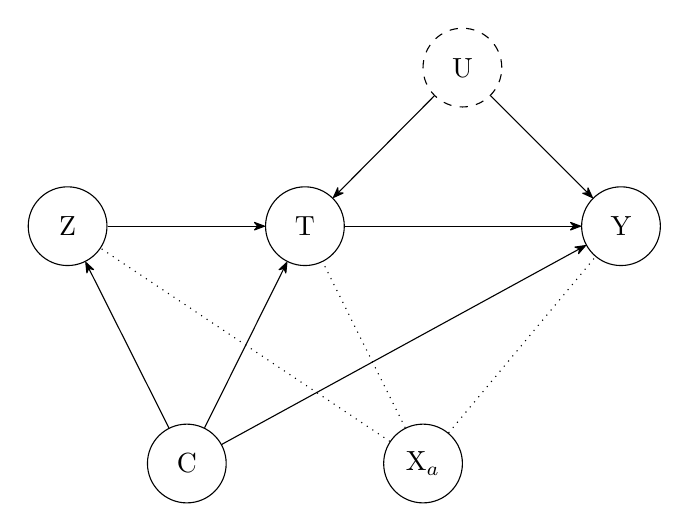
\begin{tikzpicture}[
        >={Stealth[round]},
        every node/.style={draw, circle, minimum size=1cm},
        every edge/.style={draw, ->, thick},
        node distance=2cm
    ]
    
    \node (Z) {Z};
    \node (T) [right=of Z] {T};
    \node (U) [above=of T, xshift=2cm, yshift=-1cm, dashed] {U};
    \node (XC) [below=of T, xshift=-1.5cm] {$\text{C}$};
    \node (XA) [below=of T, xshift=1.5cm] {$\text{X}_a$};
    \node (Y) [right=of T, xshift=1cm] {Y};
    
    \draw[->] (Z) -- (T);
    \draw[->] (T) -- (Y);
    \draw[->] (U) -- (T);
    \draw[->] (U) -- (Y);
    \draw[->] (XC) -- (T);
    \draw[->] (XC) -- (Z);
    \draw[->] (XC) -- (Y);
    \draw[dotted] (XA) -- (T);
    \draw[dotted] (XA) -- (Z);
    \draw[dotted] (XA) -- (Y);
    \end{tikzpicture}
    \caption{DAG of Instrumental Variable}
    \label{fig:dag_instrumental_variable}
\end{figure}
    
\subsubsection{Instrumental Variable Scenario in DML}

To adapt the DML framework to the IV setting, we need to define appropriate nuisance functions and construct an orthogonal score function suitable for the IV context.

The ideal nuisance functions in this scenario are:

\begin{align}
    & m_{\text{IV}}(C_i) = \mathbb{E}[Y_i \mid C_i],
    \label{eq:m_x_for_target_instrumental_variable} \\
    & q_{\text{IV}}(C_i) = \mathbb{E}[Z_i \mid C_i],
    \label{eq:q_z_for_instrument_instrumental_variable} \\
    & g_{\text{IV}}(C_i) = \mathbb{E}[T_i \mid C_i],
    \label{eq:g_x_for_treatment_instrumental_variable}
\end{align}

Where $m_{\text{IV}}(C_i)$ is the outcome model, capturing the expected outcome given covariates, $q_{\text{IV}}(C_i)$ is the instrument propensity score, representing the expected treatment given the instrument and covariates, and $g_{\text{IV}}(C_i)$ is the treatment model, representing the expected treatment given covariates.

The orthogonal score function for the IV scenario is different from the standard DML orthogonal score function. An appropriate orthogonal score function in the linear IV context is:

\begin{equation}
    \psi_{\text{IV}}(W_i; \tau, \eta) = \left( Y_i - m_{\text{IV}}(C_i) - \tau [T_i - g_{\text{IV}}(C_i)] \right) \left( Z_i - q_{\text{IV}}(C_i) \right),
    \label{eq:orthogonal_score_iv}
\end{equation}

\ifthenelse{\boolean{bool:showannotations}}{
\begin{colorparagraph}{tacolor}
    Is this orthogonal score function correct? I was not able to find another one that made more sense, but I would have thought that the variance of the propensity score should be dividing some of the parts of the orthogonal score function.
\end{colorparagraph}
}

In our simulations we also test the habilit of the ML models to estimate ATE under the following scenarios. In these scenarios, the superscript $\text{w}_i$ on the nuisance functions denotes the i-th scenario which involves misspecifications of the nuisance functions.

\paragraph{Inclusion of $C_i$ and $X_{a, i}$ on every nuisance function}

\begin{align}
    & m_{\text{IV}}^{\text{w}_1}(C_i) = \mathbb{E}[Y_i \mid C_i, X_{a, i}],
    \label{eq:m_x_for_target_instrumental_variable_wrong_1} \\
    & q_{\text{IV}}^{\text{w}_1}(C_i) = \mathbb{E}[Z_i \mid C_i, X_{a, i}],
    \label{eq:q_z_for_instrument_instrumental_variable_wrong_1} \\
    & g_{\text{IV}}^{\text{w}_1}(C_i) = \mathbb{E}[T_i \mid C_i, X_{a, i}],
    \label{eq:g_x_for_treatment_instrumental_variable_wrong_1}
\end{align}

Equations \eqref{eq:m_x_for_target_instrumental_variable_wrong_1}, \eqref{eq:q_z_for_instrument_instrumental_variable_wrong_1}, and \eqref{eq:g_x_for_treatment_instrumental_variable_wrong_1} represent a scenario in which one would not be aware that $X_a$ does not cause $T$, $Z$ and $Y$.

\paragraph{Only partial inclusion of $C_i$ and inclusion of $X_{a, i}$ on every nuisance function}

\begin{align}
    & m_{\text{IV}}^{\text{w}_2}(C_i^{p}, X_{a, i}) = \mathbb{E}[Y_i \mid C_i, X_{a, i}],
    \label{eq:m_x_for_target_instrumental_variable_wrong_2} \\
    & q_{\text{IV}}^{\text{w}_2}(C_i^{p}, X_{a, i}) = \mathbb{E}[Z_i \mid, C_i, X_{a, i}],
    \label{eq:q_z_for_instrument_instrumental_variable_wrong_2} \\
    & g_{\text{IV}}^{\text{w}_2}(C_i^{p}, X_{a, i}) = \mathbb{E}[T_i \mid C_i, X_{a, i}],
    \label{eq:g_x_for_treatment_instrumental_variable_wrong_2}
\end{align}

Equations \eqref{eq:m_x_for_target_instrumental_variable_wrong_2}, \eqref{eq:q_z_for_instrument_instrumental_variable_wrong_2}, and \eqref{eq:g_x_for_treatment_backdoor_adjustment_wrong_2} also represent a scenario in which one would not be aware that $X_a$ does not cause $T$ and $Y$ and also does not include all causal cofounders. $C^{p}_i$ is subset of $C_i$ included, where $C_i \in \mathbb{R}^{d_c}$ and $C^{p}_i \in \mathbb{R}^{d_{cp}}$ and $d_c > d_{cp}$.

\paragraph{$Z_i$ is treated as a normal cofounder}

\begin{align}
    & m_{\text{IV}}^{\text{w}_3}(C_i, Z_i) = \mathbb{E}[Y_i | C_i, Z_i],
    \label{eq:m_x_for_target_instrumental_variable_wrong_3}
    \\
    & g_{\text{IV}}^{\text{w}_3}(C_i, Z_i) = \mathbb{E}[T_i | C_i, Z_i],
    \label{eq:g_x_for_treatment_instrumental_variable_wrong_3}
\end{align}

Equations \eqref{eq:m_x_for_target_instrumental_variable_wrong_3} and \eqref{eq:g_x_for_treatment_instrumental_variable_wrong_3} represent a scenario in which one would treat $Z$ as a normal covariate. In this case, the orthogonal score function would be the same as in the backdoor adjustment scenario of \eqref{eq:orthogonal_score}.

\paragraph{$Z_i$ is treated as a normal cofounder and inclusion of $X_{a, i}$ on every nuisance function}

\begin{align}
    & m_{\text{IV}}^{\text{w}_4}(C_i, Z_i, X_{a, i}) = \mathbb{E}[Y_i | C_i, Z_i, X_{a, i}],
    \label{eq:m_x_for_target_instrumental_variable_wrong_3}
    \\
    & g_{\text{IV}}^{\text{w}_4}(C_i, Z_i, X_{a, i}) = \mathbb{E}[T_i | C_i, Z_i, X_{a, i}],
    \label{eq:g_x_for_treatment_instrumental_variable_wrong_3}
\end{align}

Equations \eqref{eq:m_x_for_target_instrumental_variable_wrong_3} and \eqref{eq:g_x_for_treatment_instrumental_variable_wrong_3} represent a scenario in which one would treat $Z$ as a normal covariate and is not aware that $X_a$ does not cause $T$, $Z$ and $Y$. In this case, the orthogonal score function would also be the same as in the backdoor adjustment scenario of \eqref{eq:orthogonal_score}.

\section{Simulation Methodology}

\subsection{Data Generating Process}

We define the the backdoor path scenario as the typical scenario. The frontdoor path and instrumental variable scenarios are variations of the typical scenario.

\subsubsection{Cofounders}

The cofounders are generated with multivariate normal distribution using a sparse covariance matrix $\Sigma_d$ and a vector of means $\boldsymbol{\mu}_d = \bf{0}$.

$\Sigma_d \in \mathbb{R}^{d \times d}$, where $d := d_a + d_c$. $d_a$ is the number of non-causal confounders previously represented as $X_a$ and $d_c$ is the number of causal confounders previously represented as $C$.

\begin{equation}
    \label{eq:cofounders_data_generating_process}
    X \sim \mathcal{N}_d(\boldsymbol{\mu}_d, \Sigma_d)
\end{equation}

The sparsity of the covariance matrix of the cofounders $\Sigma_d$ is determined by $\alpha_d$, which represents the probability that any covariance coefficient is zero. Larger $\alpha_d$'s result in sparser covariance matrices. To provide intuition on it, we report the average absolute correlation ${|\rho_d|}$ in the matrix.

After generating the data from the multivariate normal distribution defined as $X \in \mathbb{R}^{n \times d}$ we randomly separate the features of $X$ in $X_a$ and $C$. Following the logic specified above, $X_a \in \mathbb{R}^{n \times d_a}$ and $C \in \mathbb{R}^{n \times d_c}$.

In \eqref{eq:m_x_for_target_backdoor_adjustment_wrong_2} and \eqref{eq:g_x_for_treatment_backdoor_adjustment_wrong_2} ``Only partial inclusion of $C_i$ and inclusion of $X_{a, i}$ on every nuisance function'', after generating cofounders, treatment, and target, we select a subset of the causal confounders $C^{p}_i$ to be used in the nuisance functions. This would represent a scenario of unobserved confounders $U_i$. We define which causal confounders are not included in the nuisance function randomly, through the use of $p_u$, which represents the percentage of causal confounders not included in the nuisance functions. Meaning that $C^{p}_i \in \mathbb{R}^{n \times d_{cp}}$, where $d_{cp} = d_c - \lceil p_u \cdot d_c \rceil$.

\subsubsection{Treatment}

The probability of treatment is generated from a logic:

\begin{equation}
    \mathbb{P}[T_i] = \frac{1}{1 + e^{(-f(C_i) + \varepsilon_{t, i})}}
    \label{eq:probability_of_treatment}
\end{equation}

where $f(C_i)$ is a function of the causal confounders $C_i$ and $\varepsilon_{t, i}$ is a random error term generated from a normal distribution with mean 0 and variance $\sigma_{t}$.

$f(C_i)$ is a generic non-linear function explained in Section~\ref{subsubsec:f_c_non_linear_relationship}.

Treatment is later generated from a Bernoulli distribution with the probability of treatment from above in \eqref{eq:probability_of_treatment}.

\begin{equation}
    T_i \sim Bernoulli(\mathbb{P}[T_i])
\end{equation}

\ifthenelse{\boolean{bool:showquestions}}{
\begin{colorparagraph}{tacolor}
    Should $T_i$ follow a Bernoulli or just be a 1 or 0 based on the probability of the treatment? The second case would be something like
    \begin{equation*}
        T_i = \begin{cases}
            1 & \text{if } \mathbb{P}[Z_i] > 0.5 \\
            0 & \text{otherwise}
        \end{cases}
    \end{equation*}

    I believe Bernoulli is a better option.
\end{colorparagraph}
}

\subsubsection{Treatment Effect}

The true individual treatment effect is generated from:

\begin{equation}
    \tau_i(C_i) = f(C_i)
    \label{eq:treatment_effect}
\end{equation}

Again, $f(C_i)$ is a generic non-linear function explained in Section~\ref{subsubsec:f_c_non_linear_relationship}.

Meaning that there is heterogeneity in the treatment effect across the causal confounders $C_i$.

The true ATE (Average Treatment Effect) is the average of the treatment effect across the population:

\begin{equation}
    \tau = \mathbb{E}[\tau(C_i)] = \frac{1}{n} \sum_{i=1}^{n} \tau_i(C_i)
\end{equation}

\ifthenelse{\boolean{bool:showquestions}}{
\begin{colorparagraph}{tacolor}
    Should it be $\mathbb{E}[\tau_i(C_i)]$ or $\mathbb{E}[\tau(C_i)]$? Not very crucial, but must be checked.
\end{colorparagraph}
}

\subsubsection{Outcome}

The observed outcome for each individual is:

\begin{equation}
    Y_i = Y_{i, 0} + \tau_i(C_i) \cdot T_i + \varepsilon_{y, i}, \quad \varepsilon_{y, i} \sim \mathcal{N}(0, \sigma_{y})
    \label{eq:observed_outcome}
\end{equation}

where $Y_{i, 0}$ is the potential outcome if the treatment $T_i$ was not applied, $\tau_i(C_i)$ is the treatment effect, and $\varepsilon_{y, i}$ is a random error term generated from a normal distribution with mean 0 and variance $\sigma_{y}$.

\begin{equation}
    Y_{i, 0} = f(C_i)
    \label{eq:potential_outcome_no_treatment}
\end{equation}

Once more, $f(C_i)$ is a generic non-linear function explained in Section~\ref{subsubsec:f_c_non_linear_relationship}.

The potential outcome for treatment and control are:

\begin{equation}
    Y_i(1) = Y_{i, 0} + \tau_i(C_i), \quad Y_i(0) = Y_{i, 0},
    \label{eq:potential_outcomes}
\end{equation}

which can not be directly observed.

\subsubsection{$f(C_i)$ Non-Linear Transformation}
\label{subsubsec:f_c_non_linear_relationship}

The function $f(C_i)$, used to calculate $Y_{i, 0}$ and $\mathbb{P}[T_i]$ is a generic function composed non-linear relationships.

More specifically $f(C_i)$ is the weighted sum of of different ``$q$'' transformations in the causal confounders $C_i$:

\begin{equation}
    f(C) = \sum_{j=1}^{d_c} \left( \beta_{j} \cdot q_j(C_{j}) \right)
\end{equation}

Where $C_{j}$ is the the vector of the $j$-th causal confounder, $\beta_j$ is a random coefficient drawn from a uniform distribution $U(-1, 1)$, and $q_j(C_{j})$ is a random transformation of the $j$-th causal confounder. More specifically, the chosen transformation $q_j(C_{j})$ is randomly chosen from the following set of possible transformations:

\begin{figure}[H]
\begin{enumerate}[label=\roman*.]
    \item Linear: $q_j(C_{i, j}) = C_{i, j}$
    \item Quadratic: $q_j(C_{i, j}) = C_{i, j}^2$
    \item Cubic: $q_j(C_{i, j}) = C_{i, j}^3$
    \item Logarithmic: $q_j(C_{i, j}) = \log(|C_{i, j}| + 1)$
    \item Exponential: $q_j(C_{i, j}) = \exp(\frac{1}{5} C_{i, j})$
    \item Sine: $q_j(C_{i, j}) = \sin(C_{i, j})$
    \item Cosine: $q_j(C_{i, j}) = \cos(C_{i, j})$
    \item Indicator: $q_j(C_{i, j}) = \mathbb{I}\{C_{i, j} > 0\} - \mathbb{I}\{C_{i, j} \leq 0\}$
    \item Piecewise: $q_j(C_{i, j}) = 2 \mathbb{I}\{C_{i, j} < 0\} + \mathbb{I}\{0 \leq C_{i, j} < 1\} + \frac{1}{2} \mathbb{I}\{ C_{i, j} > 1\}$
\end{enumerate}
\end{figure}

\ifthenelse{\boolean{bool:showfrontdooradjustment}}{
\begin{colorparagraph}{tacolor}
    Should we keep the non-continuous transformations? I know that some of the theorems only apply for continuous functions.
\end{colorparagraph}
}

For each simulation, $f(C)$ is calculated with some of the specified transformation sets and $\beta$'s three times: one for the calculation of $Y_{i, 0}$, one for the calculation of $\mathbb{P}[T_i]$, and one for the calculation of $\tau_i(C_i)$.

For some simulations, we only allow for linear transformations in $f(C)$, aiming to compare performance of the DML models in a simpler setting.

\subsubsection{Parameter Tuning in the Data Generating Process}

The data generating process has some parameters that can be tuned to generate different scenarios. We present the following variations:

\begin{enumerate}[label=\roman*.]
    \item $f(C_i)$ for Treatment Probability: linear or non-linear transformations \eqref{eq:probability_of_treatment}.
    \item $f(C_i)$ for Treatment Effect: linear or non-linear transformations \eqref{eq:treatment_effect}.
    \item $f(C_i)$ for Outcome: linear or non-linear transformations \eqref{eq:potential_outcome_no_treatment}.
    \item $d_c$: number of causal confounders.
    \item $d_a$: number of non-causal confounders.
    \item $p_u$: percentage of causal confounders not included in the nuisance functions in the backdoor adjustment scenario with wrong specification (\ref{eq:m_x_for_target_backdoor_adjustment_wrong_2}, \ref{eq:g_x_for_treatment_backdoor_adjustment_wrong_2}).
    \item $n$: number of observations.
    \item $\alpha_d$: sparsity of the covariance matrix of cofounders ($X$), which is a direct cause of average absolute correlation between cofounders ${|\rho_d|}$ \eqref{eq:cofounders_data_generating_process}.
    \item $\sigma_t$: variance of the error term $\varepsilon_t$ in the treatment probability \eqref{eq:probability_of_treatment}.
    \item $\sigma_y$: variance of the error term $\varepsilon_y$ in the outcome \eqref{eq:observed_outcome}.
\end{enumerate}

\subsection{Differences in Data Generating Process for Instrumental Variable Scenario}
\label{subsec:differences_in_data_generating_process_for_instrumental_variable_scenario}

The instrumental variable scenario provides some differences in the data generating process compared to the backdoor adjustment scenario, thus also allowing for more parameters variation.

\subsubsection{Cofounders}

The cofounders are again generated from a multivariate normal distribution using a sparse covariance matrix $\Sigma_d$ and a vector of means $\boldsymbol{\mu}_d = \bf{0}$, as described in \eqref{eq:cofounders_data_generating_process}.

In this scenario, $X$ is divided in $X_a \in \mathbb{R}^{n \times d_a}$, $C \in \mathbb{R}^{n \times d_c}$, and $U \in \mathbb{R}^{n \times d_u}$, where $d := d_a + d_c + d_u$.

$U_i$ is used to generate $\mathbb{P}[T_i]$, and $\tau_i(C_i, U_i)$, and is not included in the nuisance functions.

\subsubsection{Instrument}

We define the instrument in both discrete and continuous forms. In both cases, the instrument is generated from $C_i$ but not from $U_i$.

In the discrete case:

\begin{equation}
    \mathbb{P}[Z_i] = \frac{1}{1 + e^{(-f(C_i) + \varepsilon_{z, i})}}, \quad \varepsilon_{z, i} \sim \mathcal{N}(0, \sigma_z)
    \label{eq:probability_of_instrument}
\end{equation}

\begin{equation}
    Z_i \sim Bernoulli(\mathbb{P}[Z_i])
\end{equation}

\ifthenelse{\boolean{bool:showquestions}}{
\begin{colorparagraph}{tacolor}
    Should $Z_i$ follow a Bernoulli or just be a 1 or 0 based on the probability of the instrument? The second case would be something like
    \begin{equation*}
        Z_i = \begin{cases}
            1 & \text{if } \mathbb{P}[Z_i] > 0.5 \\
            0 & \text{otherwise}
        \end{cases}
    \end{equation*}

    I believe Bernoulli is a better option.
\end{colorparagraph}
}

In the continuous case:

\begin{equation}
    Z_i = f(C_i) + \varepsilon_{z, i}, \quad \varepsilon_{z, i} \sim \mathcal{N}(0, \sigma_z)
    \label{eq:continuous_instrument}
\end{equation}

\subsubsection{Treatment}

The $\mathbb{P}[T_i]$ previously addressed in the backdoor adjustment scenario with \eqref{eq:probability_of_treatment} becomes:

\begin{equation}
    \mathbb{P}[T_i] = \frac{1}{1 + e^{(-f(C_i, U_i, Z_i) + \varepsilon_{t, i})}},
    \quad \varepsilon_{t, i} \sim \mathcal{N}(0, \sigma_t)
    \label{eq:probability_of_treatment_instrumental_variable}
\end{equation}

A similar procedure is done for the individual treatment effect from \eqref{eq:treatment_effect}:

\begin{equation}
    \tau_i(C_i, U_i) = f(C_i, U_i)
    \label{eq:treatment_effect_instrumental_variable}
\end{equation}

\ifthenelse{\boolean{bool:showquestions}}{
\begin{colorparagraph}{tacolor}
    Should the $\tau_i$ be a function of $Z_i$ as well? I am almost sure that no. I give an explanation below:
\end{colorparagraph}
}

In a standard instrumental variables (IV) framework, the key assumption is that the instrument $Z$ affects the outcome $Y$ only through its influence on the treatment $T$, thus influencing probability of treatment, but having no effect on the potential outcomes.

\subsubsection{Outcome}

Differently from the treatment, the data generating process of the outcome is not a function of the instrument $Z_i$. Nonetheless, it is influenced by the unobserved confounders $U_i$, thus still having a data generating process different from the backdoor adjustment scenario \eqref{eq:potential_outcome_no_treatment}.

\begin{align}
    Y_{i, 0} &= f(C_i, U_i) \\
    Y_i &= Y_{i, 0} + \tau_i(C_i, U_i) \cdot T_i + \varepsilon_{y, i}, \quad \varepsilon_{y, i} \sim \mathcal{N}(0, \sigma_{y})
\end{align}

\subsubsection{Parameter Tuning in the Data Generating Process for Instrumental Variable Scenario}
In the instrumental variable scenario, we have the possibility to tune all the previously mentioned parameters in \eqref{subsec:differences_in_data_generating_process_for_instrumental_variable_scenario} as well as:

\begin{enumerate}[label=\roman*.]
    \item $f(C_i)$ for Instrument: linear or non-linear transformations (\ref{eq:probability_of_instrument} and \ref{eq:continuous_instrument}).
    \item $\sigma_z$: variance of the error term $\varepsilon_z$ in the instrument generation (\ref{eq:probability_of_instrument} and \ref{eq:continuous_instrument}).
    \item $d_u$: number of unobserved confounders (which substitutes the percentage of causal confounders $p_u$ not included in the nuisance functions in the backdoor adjustment scenario with wrong specification).
\end{enumerate}

\newpage

\section{Appendix}

\subsection{Mild Regularity Conditions for Double Machine Learning}
\label{subsec:appendix_mild_regularity_conditions_for_dml}

\begin{enumerate}[label=\roman*.]
    \item Smoothness of the Target Function: The functions \( m(X) \) and \( g(X) \), representing the outcome and treatment models, should belong to a sufficiently smooth function class (e.g., Hölder class or Sobolev space). This ensures that they can be approximated well by machine learning methods.
    \item Boundedness and Regularity: The outcome \( Y \), treatment \( T \), and covariates \( X \) should have bounded support or satisfy moment conditions, such as:  
    \[
    \mathbb{E}[|Y|^2] < \infty, \quad \mathbb{E}[|T|^2] < \infty.
    \]  
    Additionally, \( m(X) \) and \( g(X) \) should have bounded derivatives in some cases.
    \item Sparsity or Complexity Control: The nuisance estimators \( \hat{m}(X) \) and \( \hat{g}(X) \) should satisfy complexity restrictions, such as sparsity in high-dimensional settings or controlled VC dimensions, to ensure valid estimation and inference.
    \item Consistency and Rates of Convergence: The nuisance estimators \( \hat{m}(X) \) and \( \hat{g}(X) \) must converge to the true \( m(X) \) and \( g(X) \) at sufficiently fast rates (typically faster than \( n^{-1/4} \) in terms of mean squared error). 
    \item Independence or Weak Dependence: Observations should be independent and identically distributed (i.i.d.) or satisfy weak dependence conditions, such as mixing properties for time-series data.
    \item Overlap Condition (Positivity): The propensity score \( \pi(X) = \mathbb{P}(T=1|X) \) must be bounded away from 0 and 1:  
    \[
    0 < c \leq \pi(X) \leq 1 - c \quad \text{for some } c > 0.
    \]
    \item Orthogonality of the Moment Function: The estimating equation or moment function used in DML should satisfy a doubly-robust property, meaning that small estimation errors in \( \hat{m}(X) \) and \( \hat{g}(X) \) do not affect the asymptotic distribution of the estimator.
    \item Cross-Fitting: Proper cross-fitting should be employed to ensure the orthogonality of the estimating equations and to avoid overfitting. This mitigates potential overfitting by using disjoint data splits for estimating nuisance parameters and evaluating the final moment function.
\end{enumerate}

\end{document}
